\documentclass[handout]{beamer}
 
\usepackage[utf8]{inputenc}
\usepackage{mathtools}
\usepackage{tikz}
\usetikzlibrary{calc}


\usetheme{CambridgeUS}
\useoutertheme{split}
\setbeamertemplate{title page}[default][colsep=-4bp,rounded=true]
 
%Information to be included in the title page:
\title{Symmetric Security Review}
\author{Rohit Musti}
\institute{CUNY - Hunter College}
\date{\today}
 
\begin{document}
 
\frame{\titlepage}

% Outline frame
\begin{frame}{Outline}
  \tableofcontents
\end{frame}

\section{One Time Pad Mechanism}

\begin{frame}[fragile]
  \frametitle{One Time Pad: Encryption}
  \begin{verbatim}
def encrypt(key, message):
    cipher_text = ""
    if len(key) != len(message):
      print("error, key is not the same length as the message")
      print("key length:", len(key))
      print("message length:", len(message))

    for i in range(len(key)):
      cipher_text += f"{key[i] != message[i]}"

    return cipher_text
  \end{verbatim}
\end{frame}

\begin{frame}[fragile]
  \frametitle{One Time Pad: Decryption}
  \begin{verbatim}
def decrypt(key, cipher_text):
    message = ""
    if len(key) != len(cipher_text):
      print("error, key is not the same length as the ciphertext")
      print("key length:", len(key))
      print("cipher_text length:", len(cipher_text))

    for i in range(len(key)):
      message += f"{key[i] != cipher_text[i]}"

    return message
  \end{verbatim}
\end{frame}

\begin{frame}
  \frametitle{One Time Pad: Decryption}
  \begin{itemize}
    \pause
    \item Encrypt example
    \pause
    \item Decrypt example
    \pause
    \item Correctness walk through
    \pause
    \item Is this a Shannon Cipher?
    \pause
    \item Security eaknesses in this example?
  \end{itemize}

\end{frame}

\section{Semantic Security}

\begin{frame}
    \frametitle{Semantic Security}
    \begin{tikzpicture}
      \pause
        \node[draw] (Adversary) at (-3, 2) {\(\mathcal{A}\)}; 
        \draw[thick] (Adversary) -- ++(0, -4); 
        \draw[thick] (Adversary) -- ++(-2, 0);
        \draw[thick] (-3, -2) -- ++(-2, 0);

      \pause
        \node[draw] (Challenger) at (3,2) {\(\mathcal{C}\)}; 
        \draw[thick] (Challenger) -- ++(0, -4);
        \draw[thick] (Challenger) -- ++(2, 0);
        \draw[thick] (3, -2) -- ++(2, 0);

      \pause
        \node[draw=none,fill=none,anchor=east, font=\footnotesize] (choice0) at ($(Adversary) + (0,-.75)$) {\(m_0, m_1 \xleftarrow[]{R} \mathcal{M}\)};
      \pause
        \draw[->,thick] ($(Adversary)+(0,-1)$) -- ($(Challenger)+(0,-1)$) node [pos=0.5,above,font=\footnotesize] {\(m_0, m_1\)};
      \pause
        \node[draw=none,fill=none,anchor=west, font=\footnotesize] (bit) at ($(Challenger) + (0,-1.45)$) {\(b \xleftarrow[]{R} \{0, 1\}, k \xleftarrow[]{R} K \)};
      \pause
        \node[draw=none,fill=none,anchor=west, font=\footnotesize] (bit) at ($(Challenger) + (0,-2.05)$) {\(E(k, m_b) = c\)};
      \pause
        \draw[->,thick] ($(Challenger)+(0,-2.5)$) -- ($(Adversary)+(0,-2.5)$) node [pos=0.5,above,font=\footnotesize] {\(c \)};
      \pause
        \draw[->,thick] ($(Adversary)+(-1,-4)$) -- ($(Adversary)+(-1,-5)$) node [pos=0.5,left,font=\footnotesize] {\(b\)};
      \end{tikzpicture}
\end{frame}
\begin{frame}
    \frametitle{Semantic Security \(\rightarrow\) Message Recovery Game}
    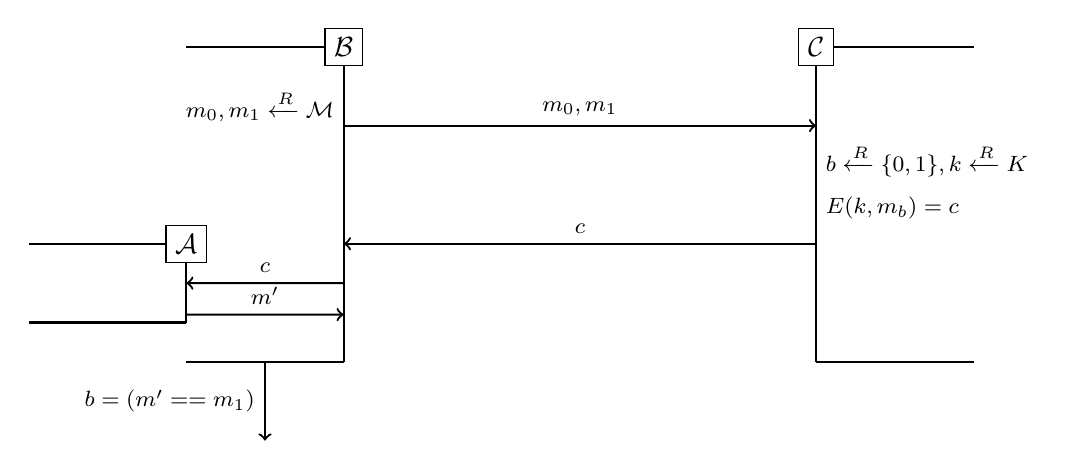
\begin{tikzpicture}


      \pause
        \node[draw] (Adversary) at (-3, 2) {\(\mathcal{B}\)}; 
        \draw[thick] (Adversary) -- ++(0, -4); 
        \draw[thick] (Adversary) -- ++(-2, 0);
        \draw[thick] (-3, -2) -- ++(-2, 0);

      \pause
        \node[draw] (Adversary2) at (-5, -0.5) {\(\mathcal{A}\)}; 
        \draw[thick] (Adversary2) -- ++(0, -1); 
        \draw[thick] (Adversary2) -- ++(-2, 0);
        \draw[thick] (-5, -1.5) -- ++(-2, 0);

      \pause
        \node[draw] (Challenger) at (3,2) {\(\mathcal{C}\)}; 
        \draw[thick] (Challenger) -- ++(0, -4);
        \draw[thick] (Challenger) -- ++(2, 0);
        \draw[thick] (3, -2) -- ++(2, 0);

      \pause
        \node[draw=none,fill=none,anchor=east, font=\footnotesize] (choice0) at ($(Adversary) + (0,-.75)$) {\(m_0, m_1 \xleftarrow[]{R} \mathcal{M}\)};
      \pause
        \draw[->,thick] ($(Adversary)+(0,-1)$) -- ($(Challenger)+(0,-1)$) node [pos=0.5,above,font=\footnotesize] {\(m_0, m_1\)};
      \pause
        \node[draw=none,fill=none,anchor=west, font=\footnotesize] (bit) at ($(Challenger) + (0,-1.45)$) {\(b \xleftarrow[]{R} \{0, 1\}, k \xleftarrow[]{R} K \)};
      \pause
        \node[draw=none,fill=none,anchor=west, font=\footnotesize] (bit) at ($(Challenger) + (0,-2.05)$) {\(E(k, m_b) = c\)};
      \pause
        \draw[->,thick] ($(Challenger)+(0,-2.5)$) -- ($(Adversary)+(0,-2.5)$) node [pos=0.5,above,font=\footnotesize] {\(c \)};

      \pause
        \draw[->,thick] ($(Adversary)+(0,-3)$) -- ($(Adversary2)+(0,-.5)$) node [pos=0.5,above,font=\footnotesize] {\(c \)};
      \pause
        \draw[->,thick] ($(Adversary2)+(0,-.9)$) -- ($(Adversary)+(0,-3.4)$) node [pos=0.5,above,font=\footnotesize] {\(m' \)};

      \pause
        \draw[->,thick] ($(Adversary)+(-1,-4)$) -- ($(Adversary)+(-1,-5)$) node [pos=0.5,left,font=\footnotesize] {\(b = (m' == m_1)\)};
      \end{tikzpicture}
\end{frame}

\section{PRG Security}

\begin{frame}
    \frametitle{PRG Security Game}
    \begin{tikzpicture}
      \pause
        \node[draw] (Adversary) at (-3, 2) {\(\mathcal{A}\)}; 
        \draw[thick] (Adversary) -- ++(0, -4); 
        \draw[thick] (Adversary) -- ++(-2, 0);
        \draw[thick] (-3, -2) -- ++(-2, 0);
      \pause

        \node[draw] (Challenger) at (3,2) {\(\mathcal{C}\)}; 
        \draw[thick] (Challenger) -- ++(0, -4);
        \draw[thick] (Challenger) -- ++(2, 0);
        \draw[thick] (3, -2) -- ++(2, 0);
      \pause

        \node[draw=none,fill=none,anchor=west, font=\footnotesize] (bit) at ($(Challenger) + (0,-0.85)$) {\(b \xleftarrow[]{R} \{0, 1\}\)};
      \pause
        \node[draw=none,fill=none,anchor=west, font=\footnotesize] (bit) at ($(Challenger) + (0,-1.45)$) {if \(b == 0 \): \(k \xleftarrow[]{R} K,\) return \(k \)};
      \pause
        \node[draw=none,fill=none,anchor=west, font=\footnotesize] (bit) at ($(Challenger) + (0,-2.05)$) {if \(b == 1 \): \(s \xleftarrow[]{R} S,\) return \(G(s) \)};
      \pause
        \draw[->,thick] ($(Challenger)+(0,-2.5)$) -- ($(Adversary)+(0,-2.5)$) node [pos=0.5,above,font=\footnotesize] {\(c \)};

      \pause
        \draw[->,thick] ($(Adversary)+(-1,-4)$) -- ($(Adversary)+(-1,-5)$) node [pos=0.5,left,font=\footnotesize] {\(b\)};
      \end{tikzpicture}
\end{frame}

\section{PRF/PRP Security}

\begin{frame}
    \frametitle{PRF Security Game: Chosen Plaintext Attack}
    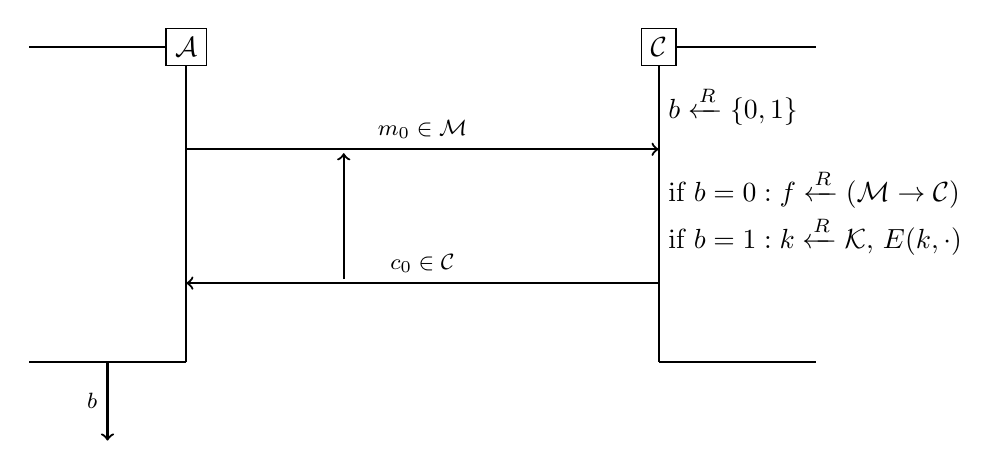
\begin{tikzpicture}
        % Public parameter:
        
        % Adversary
        \pause
        \node[draw] (Adversary) at (-3, 2) {\(\mathcal{A}\)}; 
        \draw[thick] (Adversary) -- ++(0, -4); 
        \draw[thick] (Adversary) -- ++(-2, 0);
        \draw[thick] (-3, -2) -- ++(-2, 0);
        \pause

        % Challenger
        \node[draw] (Challenger) at (3,2) {\(\mathcal{C}\)}; 
        \draw[thick] (Challenger) -- ++(0, -4);
        \draw[thick] (Challenger) -- ++(2, 0);
        \draw[thick] (3, -2) -- ++(2, 0);
        \pause

        \node[draw=none,fill=none,anchor=west] (bit) at ($(Challenger) + (0,-.75)$) {\(b \xleftarrow[]{R} \{0, 1\} \)};
        \pause
        \node[draw=none,fill=none,anchor=west] (choice0) at ($(Challenger) + (0,-1.8)$) {if \(b = 0: f \xleftarrow[]{R}(\mathcal{M} \rightarrow \mathcal{C}) \)};
        \pause
        \node[draw=none,fill=none,anchor=west] (choice1) at ($(Challenger) + (0,-2.4)$) {if \(b = 1: k \xleftarrow[]{R} \mathcal{K} \), \(E(k, \cdot )\)};
        \pause
        \draw[->,thick] ($(Adversary)+(0,-1.3)$) -- ($(Challenger)+(0,-1.3)$) node [pos=0.5,above,font=\footnotesize] {\(m_0 \in \mathcal{M} \)};
        \pause
        \draw[->,thick] ($(Challenger)+(0,-3)$) -- ($(Adversary)+(0,-3)$) node [pos=0.5,above,font=\footnotesize] {\(c_0 \in \mathcal{C} \)};
        \pause
        \draw[->,thick] ($(Adversary)+(2,-2.95)$) -- ($(Adversary)+(2,-1.35)$) node [pos=0.5,left,font=\footnotesize] {};
        \pause

        \draw[->,thick] ($(Adversary)+(-1,-4)$) -- ($(Adversary)+(-1,-5)$) node [pos=0.5,left,font=\footnotesize] {\(b\)};
      \end{tikzpicture}
\end{frame}

\section{MAC}

\begin{frame}
    \frametitle{Man in the Middle Attack}
    \pause \text{Let \(\mathcal{E} = (E, D) \) be a cipher secure against chosen plaintext attacks}\\ \pause
    \bigskip
    \begin{tikzpicture}
        \node[draw] (Adversary) at (-3, 2) {\(Alice\)}; 
        \draw[thick] (Adversary) -- ++(0, -4); 
        \draw[thick] (Adversary) -- ++(-2, 0);
        \draw[thick] (-3, -2) -- ++(-2, 0);
        
        \pause

        \node[draw] (Challenger) at (4.5,2) {\(Bob\)}; 
        \draw[thick] (Challenger) -- ++(0, -4);
        \draw[thick] (Challenger) -- ++(2, 0);
        \draw[thick] (4.5, -2) -- ++(2, 0);

        \pause

        \node[draw=none,fill=none,anchor=east, font=\footnotesize] (choice0) at ($(Adversary) + (0,-.75)$) {\(c = E(k, m)\)};

        \pause

        \draw[->,thick] ($(Adversary)+(0.25,-2)$) -- ($(Challenger)+(-0.25,-2)$) node [pos=0.5,above,font=\footnotesize] {\(c \rightarrow\) Eve \(\rightarrow c'\)};

        \pause

        \node[draw=none,fill=none,anchor=east, font=\footnotesize] (choice0) at ($(Challenger) + (2.25,-3.25)$) {\(m' = D(k, c')\)};
      \end{tikzpicture}
\end{frame}

\begin{frame}
    \frametitle{MAC Visualized}
    \begin{tikzpicture}
        \node[draw] (Adversary) at (-3, 2) {\(Alice\)}; 
        \draw[thick] (Adversary) -- ++(0, -4); 
        \draw[thick] (Adversary) -- ++(-2, 0);
        \draw[thick] (-3, -2) -- ++(-2, 0);
        
        \pause

        \node[draw] (Challenger) at (4.5,2) {\(Bob\)}; 
        \draw[thick] (Challenger) -- ++(0, -4);
        \draw[thick] (Challenger) -- ++(2, 0);
        \draw[thick] (4.5, -2) -- ++(2, 0);

        \pause

        \node[draw=none,fill=none,anchor=east, font=\footnotesize] (choice0) at ($(Adversary) + (0,-.75)$) {\(t = S(k, m)\)};

        \pause

        \draw[->,thick] ($(Adversary)+(0.25,-2)$) -- ($(Challenger)+(-0.25,-2)$) node [pos=0.5,above,font=\footnotesize] {\(c, t\)};

        \pause

        \node[draw=none,fill=none,anchor=east, font=\footnotesize] (choice0) at ($(Challenger) + (2.25,-3.25)$) {\(r = V(k,m,t)\)};
      \end{tikzpicture}
\end{frame}

\begin{frame}
    \frametitle{MAC Attack Game}
    \text{} \\
      \[ V(k,m,t) = S(k,m) == t \] \pause
    \bigskip
    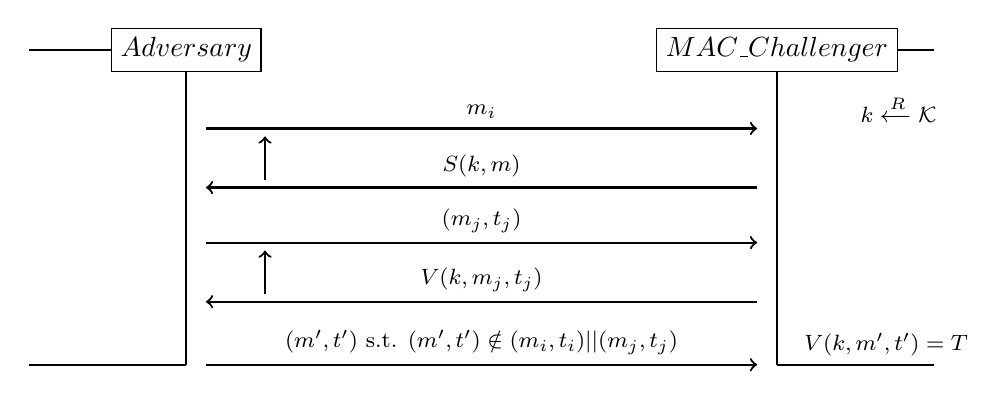
\begin{tikzpicture}
        \node[draw] (Adversary) at (-3, 2) {\(Adversary\)}; 
        \draw[thick] (Adversary) -- ++(0, -4); 
        \draw[thick] (Adversary) -- ++(-2, 0);
        \draw[thick] (-3, -2) -- ++(-2, 0);
        
        \pause

        \node[draw] (Challenger) at (4.5,2) {\(MAC\_Challenger\)}; 
        \draw[thick] (Challenger) -- ++(0, -4);
        \draw[thick] (Challenger) -- ++(2, 0);
        \draw[thick] (4.5, -2) -- ++(2, 0);

        \pause

        \node[draw=none,fill=none,anchor=east, font=\footnotesize] (choice0) at ($(Challenger) + (2.15,-.75)$) {\(k \xleftarrow{R} \mathcal{K}\)};

        \pause

        \draw[->,thick] ($(Adversary)+(0.25,-1)$) -- ($(Challenger)+(-0.25,-1)$) node [pos=0.5,above,font=\footnotesize] {\(m_i\)};

        \pause

        \draw[->,thick] ($(Challenger)+(-0.25,-1.75)$) -- ($(Adversary)+(0.25,-1.75)$) node [pos=0.5,above,font=\footnotesize] {\(S(k, m)\)};

        \pause

        \draw[->,thick] ($(Adversary)+(1,-1.65)$) -- ($(Adversary)+(1,-1.1)$);

        \pause

        \draw[->,thick] ($(Adversary)+(0.25,-2.45)$) -- ($(Challenger)+(-0.25,-2.45)$) node [pos=0.5,above,font=\footnotesize] {\((m_j,t_j)\)};

        \pause

        \draw[->,thick] ($(Challenger)+(-0.25,-3.2)$) -- ($(Adversary)+(0.25,-3.2)$) node [pos=0.5,above,font=\footnotesize] {\(V(k, m_j, t_j)\)};

        \pause

        \draw[->,thick] ($(Adversary)+(1,-3.1)$) -- ($(Adversary)+(1,-2.55)$);

        \pause

        \draw[->,thick] ($(Adversary)+(0.25,-4)$) -- ($(Challenger)+(-0.25,-4)$) node [pos=0.5,above,font=\footnotesize] {\((m', t')\) s.t. \((m',t') \notin (m_i, t_i) || (m_j, t_j)\)};
        
        \pause

        \node[draw=none,fill=none,anchor=east, font=\footnotesize] (choice0) at ($(Challenger) + (2.55,-3.75)$) {\(V(k, m', t') = T\)};
      \end{tikzpicture} 
\end{frame}

\section{Authenticated Encryption}


\begin{frame}
    \frametitle{Cipher Text Integrity Game}
    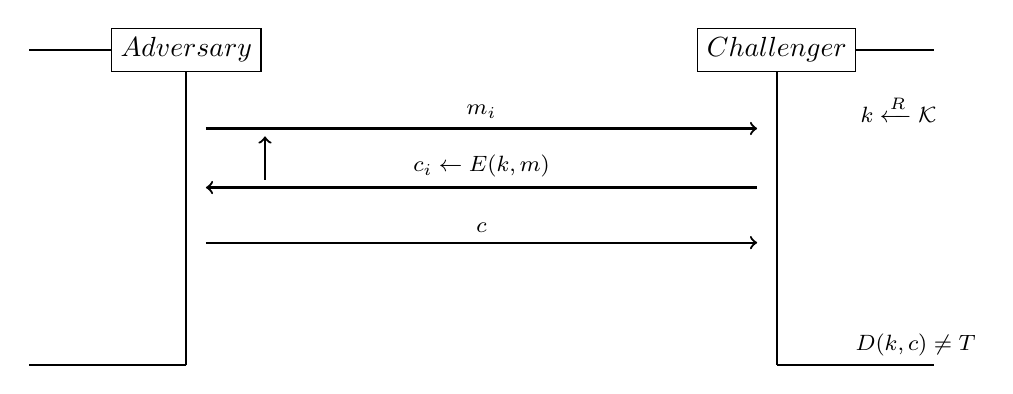
\begin{tikzpicture}
        \node[draw] (Adversary) at (-3, 2) {\(Adversary\)}; 
        \draw[thick] (Adversary) -- ++(0, -4); 
        \draw[thick] (Adversary) -- ++(-2, 0);
        \draw[thick] (-3, -2) -- ++(-2, 0);
        
        \pause

        \node[draw] (Challenger) at (4.5,2) {\(Challenger\)}; 
        \draw[thick] (Challenger) -- ++(0, -4);
        \draw[thick] (Challenger) -- ++(2, 0);
        \draw[thick] (4.5, -2) -- ++(2, 0);

        \pause

        \node[draw=none,fill=none,anchor=east, font=\footnotesize] (choice0) at ($(Challenger) + (2.15,-.75)$) {\(k \xleftarrow{R} \mathcal{K}\)};

        \pause

        \draw[->,thick] ($(Adversary)+(0.25,-1)$) -- ($(Challenger)+(-0.25,-1)$) node [pos=0.5,above,font=\footnotesize] {\(m_i\)};

        \pause

        \draw[->,thick] ($(Challenger)+(-0.25,-1.75)$) -- ($(Adversary)+(0.25,-1.75)$) node [pos=0.5,above,font=\footnotesize] {\(c_i \leftarrow E(k, m)\)};

        \pause

        \draw[->,thick] ($(Adversary)+(1,-1.65)$) -- ($(Adversary)+(1,-1.1)$);

        \pause

        \draw[->,thick] ($(Adversary)+(0.25,-2.45)$) -- ($(Challenger)+(-0.25,-2.45)$) node [pos=0.5,above,font=\footnotesize] {\(c\)};


        \node[draw=none,fill=none,anchor=east, font=\footnotesize] (choice0) at ($(Challenger) + (2.65,-3.75)$) {\(D(k, c) \neq T \) };
      \end{tikzpicture} 
\end{frame}


\end{document}